% =====================================================================
% ELMED219: Pasient-likhetsnettverk (PSN)
% Beamer-presentasjon - Momentliste P01-P08
% =====================================================================
\documentclass[aspectratio=169, 10pt]{beamer}

% =====================================================================
% PAKKER
% =====================================================================
\usepackage[utf8]{inputenc}
\usepackage[T1]{fontenc}
\usepackage[norsk]{babel}
\usepackage{graphicx}
\usepackage{tikz}
\usetikzlibrary{shapes.geometric, arrows, positioning, calc}
\usepackage{booktabs}
\usepackage{amsmath}
\usepackage{fontawesome5}

% =====================================================================
% TEMA OG FARGER
% =====================================================================
\usetheme{Madrid}
\usecolortheme{beaver}

% Farger for TikZ-diagrammer
\definecolor{uibblue}{RGB}{0, 61, 115}
\definecolor{uibred}{RGB}{175, 28, 44}

% =====================================================================
% TITTELINFO
% =====================================================================
\title{Pasient-likhetsnettverk (PSN)}
\subtitle{ELMED219: Momentliste P01--P08}
\author{ELMED219}
\date{Vår 2026}

% =====================================================================
% DOKUMENT
% =====================================================================
\begin{document}

% Tittelside
\begin{frame}
    \titlepage
\end{frame}

% Innholdsfortegnelse
\begin{frame}{Oversikt}
    \tableofcontents
\end{frame}

% =====================================================================
% SEKSJON: Grunnleggende om PSN
% =====================================================================
\section{Grunnleggende om PSN}

\begin{frame}{P01: Forklare konseptet pasient-likhetsnettverk (PSN)}
    \begin{columns}[T]
        \begin{column}{0.55\textwidth}
            \textbf{Hva er et pasient-likhetsnettverk?}
            \begin{itemize}
                \item En \textbf{graf} der hver node representerer en pasient
                \item \textbf{Kanter} forbinder pasienter som ligner hverandre
                \item Likhet basert på kliniske variabler, biomarkører, genetikk
            \end{itemize}
            
            \vspace{0.3cm}
            \textbf{Hovedidé:}
            \begin{itemize}
                \item Pasienter med lignende profiler grupperes sammen
                \item Avdekker naturlige subgrupper i pasientpopulasjonen
                \item Grunnlag for pasient-stratifisering
            \end{itemize}
        \end{column}
        \begin{column}{0.42\textwidth}
            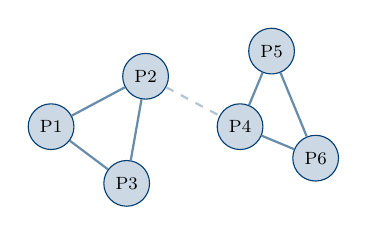
\begin{tikzpicture}[scale=0.8, transform shape]
                \tikzstyle{patient} = [circle, draw=uibblue, fill=uibblue!20, minimum size=0.7cm, font=\footnotesize]
                \tikzstyle{edge} = [draw, thick, uibblue!60]
                
                \node[patient] (p1) at (0,0) {P1};
                \node[patient] (p2) at (1.5,0.8) {P2};
                \node[patient] (p3) at (1.2,-0.9) {P3};
                \node[patient] (p4) at (3,0) {P4};
                \node[patient] (p5) at (3.5,1.2) {P5};
                \node[patient] (p6) at (4.2,-0.5) {P6};
                
                \draw[edge] (p1) -- (p2);
                \draw[edge] (p1) -- (p3);
                \draw[edge] (p2) -- (p3);
                \draw[edge] (p4) -- (p5);
                \draw[edge] (p4) -- (p6);
                \draw[edge] (p5) -- (p6);
                \draw[edge, dashed, uibblue!30] (p2) -- (p4);
            \end{tikzpicture}
            
            \vspace{0.3cm}
            \footnotesize\textit{To pasientgrupper med sterk intern likhet}
        \end{column}
    \end{columns}
\end{frame}

\begin{frame}{P02: Beskrive hvordan PSN kan støtte presisjonsmedisin}
    \begin{block}{Presisjonsmedisin}
        Tilpasse behandling til den individuelle pasienten basert på deres unike profil -- ikke ``one size fits all''
    \end{block}
    
    \vspace{0.3cm}
    \textbf{PSN støtter presisjonsmedisin ved å:}
    \begin{enumerate}
        \item \textbf{Identifisere subgrupper} -- Finne pasienter med lignende sykdomsmekanismer
        \item \textbf{Predikere behandlingsrespons} -- ``Pasienter som ligner deg responderte godt på X''
        \item \textbf{Oppdage ukjente sammenhenger} -- Avdekke mønstre på tvers av datatyper
        \item \textbf{Integrere heterogene data} -- Kombinere klinikk, omikk, avbildning
    \end{enumerate}
    
    \vspace{0.3cm}
    \begin{alertblock}{Eksempel: IBS-studien}
        I Lab 1 bruker vi PSN på IBS-pasienter for å undersøke sammenhenger mellom tarmsymptomer, hjerneavbildning (MRI) og kognitive funksjoner.
    \end{alertblock}
\end{frame}

% =====================================================================
% SEKSJON: Likhetsberegning
% =====================================================================
\section{Likhetsberegning}

\begin{frame}{P03: Beregne likhet mellom pasienter}
    \textbf{Vanlige avstandsmål:}
    
    \vspace{0.3cm}
    \begin{columns}[T]
        \begin{column}{0.48\textwidth}
            \textbf{Euklidsk avstand:}
            \[
            d_E = \sqrt{\sum_{i=1}^{n}(x_i - y_i)^2}
            \]
            \begin{itemize}
                \item Rett linje mellom punkter
                \item Følsom for skala
                \item God for kontinuerlige data
            \end{itemize}
            
            \vspace{0.3cm}
            \textbf{Manhattan avstand:}
            \[
            d_M = \sum_{i=1}^{n}|x_i - y_i|
            \]
            \begin{itemize}
                \item ``Byblokk''-avstand
                \item Mer robust mot uteliggere
            \end{itemize}
        \end{column}
        \begin{column}{0.48\textwidth}
            \textbf{Gower-avstand:}
            \[
            d_G = \frac{1}{n}\sum_{i=1}^{n}d_i(x_i, y_i)
            \]
            \begin{itemize}
                \item Håndterer \textbf{blandede datatyper}
                \item Numeriske, kategoriske, binære
                \item Normaliserer automatisk
                \item Ideell for kliniske data!
            \end{itemize}
            
            \vspace{0.3cm}
            \begin{block}{Konvertering}
                $\text{likhet} = 1 - \text{avstand}$ \\
                (når avstand er normalisert til [0,1])
            \end{block}
        \end{column}
    \end{columns}
\end{frame}

\begin{frame}{P04: Konstruere et PSN fra en pasient-feature-matrise}
    \textbf{Steg-for-steg prosess:}
    
    \begin{enumerate}
        \item \textbf{Organiser data:} Pasient $\times$ Feature-matrise
        \begin{center}
            \footnotesize
            \begin{tabular}{l|ccc}
                \toprule
                Pasient & Alder & BMI & Symptom-score \\
                \midrule
                P1 & 45 & 24.5 & 7 \\
                P2 & 42 & 25.1 & 8 \\
                P3 & 67 & 31.2 & 3 \\
                \bottomrule
            \end{tabular}
        \end{center}
        
        \item \textbf{Normaliser/standardiser:} Gjør variabler sammenlignbare
        
        \item \textbf{Beregn likhetsmatrise:} Alle par av pasienter
        
        \item \textbf{Velg terskelverdi:} Bestem når to pasienter er ``like nok''
        
        \item \textbf{Opprett kanter:} Forbind pasienter med likhet $>$ terskel
        
        \item \textbf{Bygg graf:} Bruk NetworkX for å lage nettverket
    \end{enumerate}
    
    \begin{block}{Python-kode (konseptuelt)}
        \texttt{G = nx.Graph()} \\
        \texttt{for i, j: if similarity[i,j] > threshold: G.add\_edge(i,j)}
    \end{block}
\end{frame}

\begin{frame}{P05: Velge terskelverdi for kantoppretting i PSN}
    \textbf{Utfordringen:}
    \begin{itemize}
        \item For lav terskel $\rightarrow$ For mange kanter, alle pasienter koblet
        \item For høy terskel $\rightarrow$ For få kanter, isolerte noder
    \end{itemize}
    
    \vspace{0.3cm}
    \textbf{Strategier for terskelvalg:}
    \begin{enumerate}
        \item \textbf{Persentilbasert:} Behold topp 5--10\% av kantene
        \item \textbf{k-nærmeste naboer (k-NN):} Hver node kobles til k nærmeste
        \item \textbf{Statistisk terskel:} $\mu + 1.5\sigma$ av likhetsfordelingen
        \item \textbf{Visuell inspeksjon:} Prøv ulike verdier og visualiser
    \end{enumerate}
    
    \vspace{0.3cm}
    \begin{columns}[T]
        \begin{column}{0.48\textwidth}
            \begin{alertblock}{For mange kanter}
                Mister subgruppestruktur, vanskelig å tolke
            \end{alertblock}
        \end{column}
        \begin{column}{0.48\textwidth}
            \begin{alertblock}{For få kanter}
                Mister informasjon, fragmentert nettverk
            \end{alertblock}
        \end{column}
    \end{columns}
\end{frame}

% =====================================================================
% SEKSJON: Analyse av PSN
% =====================================================================
\section{Analyse av PSN}

\begin{frame}{P06: Identifisere pasientsubgrupper via community detection}
    \textbf{Community detection i PSN:}
    \begin{itemize}
        \item Finner naturlige grupperinger av pasienter
        \item Pasienter i samme gruppe ligner hverandre mer enn de ligner andre
    \end{itemize}
    
    \vspace{0.3cm}
    \textbf{Louvain-algoritmen (fra N09):}
    \begin{enumerate}
        \item Optimaliserer \textbf{modularitet} -- intern tetthet vs. eksterne koblinger
        \item Hierarkisk: Finner grupper på flere nivåer
        \item Rask og skalerbar
    \end{enumerate}
    
    \vspace{0.3cm}
    \textbf{Klinisk tolkning:}
    \begin{itemize}
        \item Hver community = potensiell pasientsubtype
        \item Undersøk karakteristika for hver gruppe
        \item Sammenlign utfall og behandlingsrespons
    \end{itemize}
    
    \begin{block}{NetworkX/python-louvain}
        \texttt{import community} \\
        \texttt{partition = community.best\_partition(G)}
    \end{block}
\end{frame}

% =====================================================================
% SEKSJON: Avanserte temaer
% =====================================================================
\section{Avanserte temaer}

\begin{frame}{P07: Fordeler og begrensninger ved PSN-tilnærmingen}
    \begin{columns}[T]
        \begin{column}{0.48\textwidth}
            \textbf{\textcolor{green!60!black}{Fordeler:}}
            \begin{itemize}
                \item \faCheck~Intuitivt og visuelt
                \item \faCheck~Integrasjon av ulike datatyper
                \item \faCheck~Ingen antakelse om underliggende fordelinger
                \item \faCheck~Oppdager ikke-lineære sammenhenger
                \item \faCheck~Nettverksanalyse-verktøy kan anvendes
                \item \faCheck~Pasient-sentrert perspektiv
            \end{itemize}
        \end{column}
        \begin{column}{0.48\textwidth}
            \textbf{\textcolor{uibred}{Begrensninger:}}
            \begin{itemize}
                \item \faTimes~Valg av likhetsmål og terskel er kritisk
                \item \faTimes~Skalerer dårlig til store datasett
                \item \faTimes~Manglende data kan være problematisk
                \item \faTimes~Tolkningsutfordringer
                \item \faTimes~Ikke alltid replikerbart
                \item \faTimes~Krever domeneekspertise
            \end{itemize}
        \end{column}
    \end{columns}
    
    \vspace{0.5cm}
    \begin{block}{Oppsummering}
        PSN er et kraftig verktøy for eksplorativ analyse og hypotesegenerering, men resultater bør valideres med uavhengige data og metoder.
    \end{block}
\end{frame}

\begin{frame}{P08: Multimodal PSN (integrering av ulike datatyper)}
    \textbf{Multimodal PSN:}
    \begin{itemize}
        \item Kombinerer data fra \textbf{flere kilder/modaliteter}
        \item Eksempler: Klinikk + Genetikk + Avbildning
    \end{itemize}
    
    \vspace{0.3cm}
    \textbf{Integrasjonsstrategier:}
    \begin{enumerate}
        \item \textbf{Tidlig fusjon:} Kombiner alle features før likhetsberegning
        \item \textbf{Sen fusjon:} Lag separate PSN, kombiner etterpå
        \item \textbf{Mellomliggende fusjon:} Vektet kombinasjon av likhetsmatriser
    \end{enumerate}
    
    \vspace{0.3cm}
    \textbf{Eksempel fra Lab 1 (IBS-studie):}
    \begin{itemize}
        \item \textbf{Kliniske data:} Symptomscorer, demografi
        \item \textbf{MRI-data:} Hjerneavbildning (konnektivitet, volum)
        \item \textbf{Kognitive data:} Testresultater
        \item $\rightarrow$ Integrert PSN for helhetlig pasientprofilering
    \end{itemize}
    
    \begin{block}{Verdi av multimodal PSN}
        Fanger opp kompleksiteten i pasientpopulasjoner som ikke synes i enkeltmodaliteter alene.
    \end{block}
\end{frame}

% =====================================================================
% OPPSUMMERING
% =====================================================================
\section*{Oppsummering}

\begin{frame}{Oppsummering: PSN}
    \textbf{Nøkkelpunkter:}
    \begin{itemize}
        \item \textbf{P01:} PSN = Graf der noder er pasienter, kanter er likhet
        \item \textbf{P02:} Støtter presisjonsmedisin via subgruppeidentifikasjon
        \item \textbf{P03:} Likhetsmål: Euklidsk, Manhattan, Gower
        \item \textbf{P04:} Konstruksjon: Feature-matrise $\rightarrow$ Likhet $\rightarrow$ Graf
        \item \textbf{P05:} Terskelvalg er kritisk for nettverksstruktur
        \item \textbf{P06:} Community detection (Louvain) for subgrupper
        \item \textbf{P07:} Fordeler vs. begrensninger må avveies
        \item \textbf{P08:} Multimodal PSN integrerer heterogene data
    \end{itemize}
    
    \vspace{0.3cm}
    \begin{block}{Lab 1 -- Praktisk erfaring}
        Konstruer og analyser PSN med ekte kliniske data (IRIS, IBS, WAIS-IV) ved hjelp av Python og NetworkX.
    \end{block}
\end{frame}

\end{document}
